%==============================================================================
% PAPER 6, CHAPTER 3: Metamaterial Spacetime Engineering
%==============================================================================

\chapter{Metamaterial Spacetime Engineering}

%------------------------------------------------------------------------------
% Opening Narrative: Veselago's Vision
%------------------------------------------------------------------------------

In 1968, Viktor Veselago published a remarkable theoretical paper in the Soviet
journal \emph{Uspekhi Fizicheskikh Nauk}, asking a question that seemed almost
frivolous: what would happen if both the permittivity $\varepsilon$ and
permeability $\mu$ of a material were simultaneously negative? At the time,
no such materials existed in nature. The dielectric constant $\varepsilon$
describes how a material responds to electric fields, while the magnetic
permeability $\mu$ characterizes its response to magnetic fields. For all
known substances, both quantities were positive.

\marginhistory{Veselago's 1968 paper was largely ignored for three decades
until Pendry's 1996 work on photonic crystals revived interest in artificial
electromagnetic materials. The term ``metamaterial'' was coined around 2000.}

Veselago showed that such a hypothetical substance would exhibit extraordinary
properties: light would refract negatively at interfaces, bending to the
``wrong'' side of the normal. The Doppler shift would reverse direction.
Cherenkov radiation would emerge backward. Most remarkably, a flat slab of
negative-index material could function as a perfect lens, focusing not just
propagating waves but also the evanescent fields that carry subwavelength
information.

For thirty years, Veselago's ideas remained a theoretical curiosity. Then, in
2000, John Pendry and David Smith independently demonstrated that arrays of
conducting wires and split-ring resonators could achieve effective negative
$\varepsilon$ and $\mu$ in the microwave regime. The age of metamaterials had
begun.

\margincomp{Modern computational electromagnetic solvers like COMSOL and CST
enable the design of metamaterial unit cells with prescribed effective
parameters. Topology optimization algorithms can discover non-intuitive
geometries that classical design would miss.}

What Veselago and his intellectual descendants had discovered was something
far more profound than mere optical trickery. They had found a way to
engineer the effective \emph{spacetime metric} experienced by electromagnetic
waves. By sculpting the material parameters $\varepsilon(\mathbf{r},\omega)$
and $\mu(\mathbf{r},\omega)$ as functions of position and frequency, one could
make light propagate as if through curved space---even though the physical
geometry remained Euclidean. The material becomes a simulator of spacetime
itself.

\margincaution{The perfect lens requires exactly $\varepsilon = \mu = -1$,
with zero loss. Real materials have absorption, limiting resolution to roughly
$\lambda/3$ rather than true subwavelength imaging. Loss compensation using
gain media remains an active research challenge.}

This chapter explores how metamaterial engineering realizes the geometric
principles developed in earlier papers. We begin with the formal connection
between material parameters and effective metrics, then examine transformation
optics, acoustic analogs, and fractal antenna designs that exploit
self-similarity across scales.

%------------------------------------------------------------------------------
% Section 1: Effective Metric from Material Properties
%------------------------------------------------------------------------------

\section{Effective Metric from Material Properties}

Maxwell's equations in a medium with permittivity $\varepsilon(\mathbf{r},\omega)$
and permeability $\mu(\mathbf{r},\omega)$ can be rewritten in a form that
reveals their geometric character. Consider the wave equation for the electric
field in a non-magnetic, isotropic medium:

\marginmath{The derivation starts from $\nabla \times (\nabla \times \mathbf{E})
= -\partial_t (\nabla \times \mathbf{B}) = -\mu_0 \varepsilon(\mathbf{r})
\partial_t^2 \mathbf{E}$. For spatially varying $\varepsilon$, this becomes
a wave equation with position-dependent wave speed.}

\begin{equation}
\nabla^2 \mathbf{E} - \nabla(\nabla \cdot \mathbf{E}) =
\varepsilon(\mathbf{r}) \mu_0 \frac{\partial^2 \mathbf{E}}{\partial t^2}
\end{equation}

This can be recast as a wave equation on an effective Riemannian manifold. For
a time-harmonic field $\mathbf{E} = \mathbf{E}_0 e^{-i\omega t}$ propagating
through a medium with spatially varying but isotropic permittivity, the Helmholtz
equation becomes:

\begin{equation}
\nabla^2 \mathbf{E}_0 + k_0^2 \varepsilon_r(\mathbf{r}) \mathbf{E}_0 = 0
\end{equation}

where $k_0 = \omega/c$ is the free-space wavenumber. Now perform a coordinate
transformation $x^i \to x'^i$. Under this transformation, the Laplacian becomes:

\marginphysics{The coordinate transformation induces a metric tensor
$g_{ij}' = (\partial x^k / \partial x'^i)(\partial x^l / \partial x'^j) g_{kl}$.
Maxwell's equations in the new coordinates look identical to the original
equations, but with transformed material parameters.}

\begin{equation}
\nabla'^2 = g'^{ij} \nabla'_i \nabla'_j =
\frac{1}{\sqrt{g'}} \partial_i \left( \sqrt{g'} g'^{ij} \partial_j \right)
\end{equation}

where $g' = \det(g'_{ij})$ is the determinant of the metric tensor in the new
coordinates. Matching this with the Helmholtz equation reveals that the
transformed permittivity and permeability must be:

\begin{equation}
\varepsilon'^{ij} = \mu'^{ij} = \frac{1}{\det(\mathbf{J})}
\mathbf{J} \mathbf{J}^T
\label{eq:transformation_optics}
\end{equation}

where $\mathbf{J}$ is the Jacobian matrix of the coordinate transformation.
This is the fundamental result of \emph{transformation optics}: a coordinate
transformation in virtual space corresponds to a material prescription in
physical space.

\marginxref{The connection to general relativity is profound. Einstein's
equivalence principle states that gravity is indistinguishable from
acceleration. Here, material structure is indistinguishable from spatial
curvature---from the perspective of light.}

\subsection{Dispersion Engineering}

The frequency dependence of $\varepsilon(\omega)$ and $\mu(\omega)$ enables
control over wave propagation at different frequencies. Near resonances, the
material parameters can become negative or exhibit strong dispersion. Consider
a Drude model for the permittivity:

\begin{equation}
\varepsilon(\omega) = \varepsilon_\infty -
\frac{\omega_p^2}{\omega^2 + i\gamma\omega}
\end{equation}

where $\omega_p$ is the plasma frequency and $\gamma$ is the damping rate.
For $\omega < \omega_p$, the permittivity is negative. Similarly, a resonant
magnetic response gives:

\margindim{The plasma frequency is $\omega_p = \sqrt{n e^2 / (m \varepsilon_0)}$
for electron density $n$. For metals, $\omega_p \sim 10^{16}$ rad/s (UV range).
For artificial wire arrays with effective electron density, $\omega_p$ can be
tuned to GHz frequencies.}

\begin{equation}
\mu(\omega) = 1 + \frac{F\omega^2}{\omega_0^2 - \omega^2 - i\gamma\omega}
\end{equation}

where $\omega_0$ is the resonance frequency and $F$ is the oscillator strength.
For $\omega > \omega_0$, this can become negative.

The following diagram shows the typical dispersion behavior:

\begin{center}
\begin{tikzpicture}[scale=1.0]
  % Axes
  \draw[->] (0,0) -- (8,0) node[right] {$\omega$ (rad/s)};
  \draw[->] (0,-2.5) -- (0,2.5) node[above] {$\varepsilon(\omega), \mu(\omega)$};

  % Zero line
  \draw[dashed, gray] (0,0) -- (8,0);

  % Epsilon curve (Drude)
  \draw[thick, blue] plot[smooth, domain=0.5:7.5]
    (\x, {2 - 9/(\x*\x)}) node[right] {$\varepsilon(\omega)$};

  % Mu curve (resonant)
  \draw[thick, red] plot[smooth, domain=0.5:7.5]
    (\x, {1 + 4/((4-\x)*(4-\x) + 0.5)}) node[right] {$\mu(\omega)$};

  % Mark plasma frequency
  \draw[dotted] (3,0) -- (3,-2.5);
  \node[below] at (3,-2.5) {$\omega_p$};

  % Mark resonance
  \draw[dotted] (4,0) -- (4,2.5);
  \node[above] at (4,2.5) {$\omega_0$};

  % Shaded region where both negative
  \fill[green, opacity=0.2] (3,-2) rectangle (3.8,0);
  \node[text width=2cm, align=center] at (3.4,-1.5) {\small both\\negative};

\end{tikzpicture}
\end{center}

\marginex{Example: A split-ring resonator array achieves negative $\mu$ near
1 GHz with dimensions $\sim 1$ cm. Combined with a wire array (negative
$\varepsilon$ below $\sim 2$ GHz), this creates a negative-index band from
0.9--1.1 GHz. The effective refractive index is $n = -\sqrt{\varepsilon\mu}$.}

%------------------------------------------------------------------------------
% Section 2: Transformation Optics
%------------------------------------------------------------------------------

\section{Transformation Optics and Cloaking}

Equation~\ref{eq:transformation_optics} provides a recipe for designing
metamaterials: choose a desired coordinate transformation, compute the Jacobian,
and synthesize materials with the prescribed $\varepsilon$ and $\mu$ tensors.
This is the principle of \emph{transformation optics}, pioneered by Pendry and
Leonhardt in 2006.

\subsection{The Pendry Cloak}

Consider a spherical coordinate transformation that compresses the region
$0 < r < a$ into a shell $b < r' < a$, while leaving $r > a$ unchanged:

\marginphysics{The transformation creates a ``hole'' in coordinate space from
$0 < r < b$. Light rays cannot enter this region because they follow geodesics
in the transformed space. The region becomes invisible to external observers.}

\begin{equation}
r' = b + \frac{a-b}{a} r, \quad \theta' = \theta, \quad \phi' = \phi
\end{equation}

The Jacobian of this transformation yields the required material parameters in
the cloak shell ($b < r < a$):

\begin{align}
\varepsilon_r &= \mu_r = \frac{r' - b}{r'} \\
\varepsilon_\theta &= \mu_\theta = \frac{r'}{r' - b} \\
\varepsilon_\phi &= \mu_\phi = \frac{r'}{r' - b}
\end{align}

At the inner boundary $r' = b$, the radial parameters vanish while the
tangential parameters diverge---a challenging prescription for real materials.
Nevertheless, simplified cloaks using reduced parameters have been demonstrated
experimentally.

\begin{center}
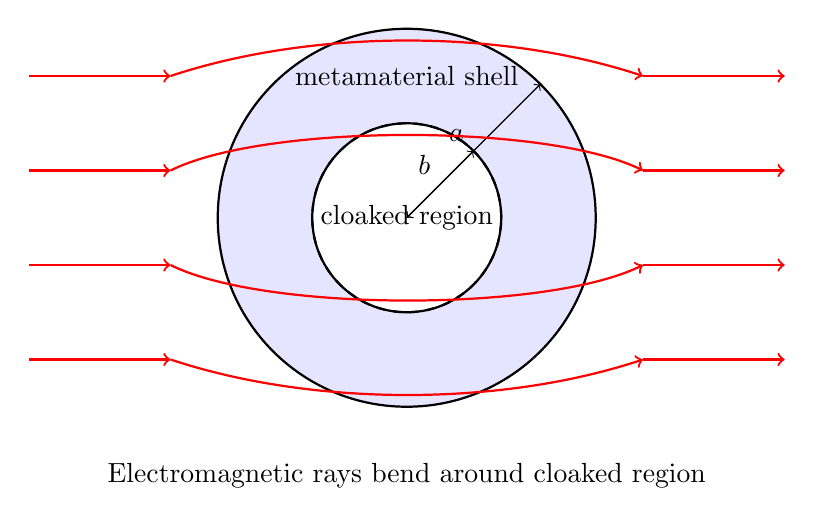
\begin{tikzpicture}[scale=1.2]
  % Draw cloak shell
  \draw[thick, fill=blue!10] (0,0) circle (2cm);
  \draw[thick, fill=white] (0,0) circle (1cm);
  \draw[thick, dashed] (0,0) circle (1cm);

  % Labels
  \node at (0,0) {cloaked region};
  \node at (0,1.5) {metamaterial shell};
  \draw[<->] (0,0) -- (0.707,0.707) node[midway, above left] {$b$};
  \draw[<->] (0,0) -- (1.414,1.414) node[midway, above left] {$a$};

  % Incoming rays
  \draw[->, thick, red] (-4,1.5) -- (-2.5,1.5);
  \draw[->, thick, red] (-4,0.5) -- (-2.5,0.5);
  \draw[->, thick, red] (-4,-0.5) -- (-2.5,-0.5);
  \draw[->, thick, red] (-4,-1.5) -- (-2.5,-1.5);

  % Bent rays around cloak
  \draw[->, thick, red] (-2.5,1.5) .. controls (-1,2) and (1,2) .. (2.5,1.5);
  \draw[->, thick, red] (-2.5,0.5) .. controls (-1.5,1) and (1.5,1) .. (2.5,0.5);
  \draw[->, thick, red] (-2.5,-0.5) .. controls (-1.5,-1) and (1.5,-1) .. (2.5,-0.5);
  \draw[->, thick, red] (-2.5,-1.5) .. controls (-1,-2) and (1,-2) .. (2.5,-1.5);

  % Exiting rays
  \draw[->, thick, red] (2.5,1.5) -- (4,1.5);
  \draw[->, thick, red] (2.5,0.5) -- (4,0.5);
  \draw[->, thick, red] (2.5,-0.5) -- (4,-0.5);
  \draw[->, thick, red] (2.5,-1.5) -- (4,-1.5);

  \node[below] at (0,-2.5) {Electromagnetic rays bend around cloaked region};
\end{tikzpicture}
\end{center}

\subsection{The Pendry Perfect Lens}

A slab of material with $\varepsilon = \mu = -1$ acts as a perfect lens,
focusing both propagating and evanescent waves. For a slab of thickness $d$,
an object at distance $z_0$ from one face produces an image at distance
$z_i = d - z_0$ from the other face.

\marginmath{The transfer matrix for a slab with $n = -1$ is
$\mathbf{M} = \begin{pmatrix} \cos(kd) & -i\sin(kd) \\ -i\sin(kd) & \cos(kd) \end{pmatrix}$
where $k = \omega/c$ for $n=1$ becomes $k = -\omega/c$ for $n=-1$. The
negative propagation phase exactly reverses diffraction.}

More remarkably, evanescent waves with transverse wavevector $k_\perp > k_0$
(which decay exponentially in free space) are amplified in the negative-index
slab, reconstructing subwavelength features at the image plane.

\begin{center}
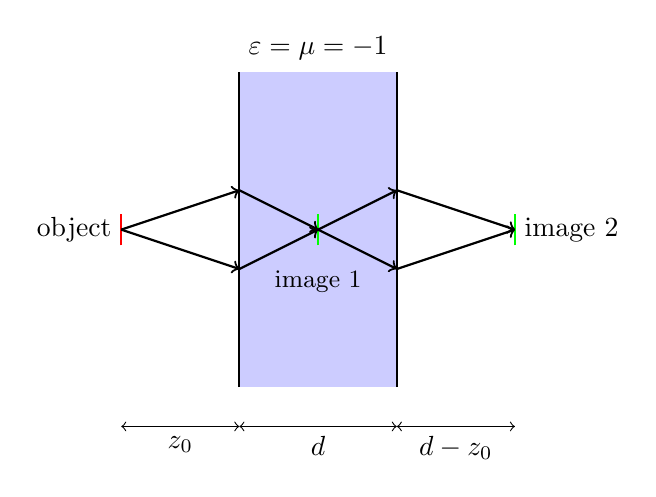
\begin{tikzpicture}[scale=1.0]
  % Slab
  \fill[blue!20] (2,0) rectangle (4,4);
  \draw[thick] (2,0) -- (2,4);
  \draw[thick] (4,0) -- (4,4);
  \node at (3,4.3) {$\varepsilon = \mu = -1$};

  % Object
  \draw[thick, red] (0.5,1.8) -- (0.5,2.2);
  \node[left] at (0.5,2) {object};

  % Image 1 (inside slab)
  \draw[thick, green] (3,1.8) -- (3,2.2);
  \node[below] at (3,1.6) {\small image 1};

  % Image 2 (outside slab)
  \draw[thick, green] (5.5,1.8) -- (5.5,2.2);
  \node[right] at (5.5,2) {image 2};

  % Ray paths
  \draw[->, thick] (0.5,2) -- (2,2.5);
  \draw[->, thick] (2,2.5) -- (3,2);
  \draw[->, thick] (3,2) -- (4,1.5);
  \draw[->, thick] (4,1.5) -- (5.5,2);

  \draw[->, thick] (0.5,2) -- (2,1.5);
  \draw[->, thick] (2,1.5) -- (3,2);
  \draw[->, thick] (3,2) -- (4,2.5);
  \draw[->, thick] (4,2.5) -- (5.5,2);

  % Dimensions
  \draw[<->] (0.5,-0.5) -- (2,-0.5) node[midway, below] {$z_0$};
  \draw[<->] (2,-0.5) -- (4,-0.5) node[midway, below] {$d$};
  \draw[<->] (4,-0.5) -- (5.5,-0.5) node[midway, below] {$d-z_0$};
\end{tikzpicture}
\end{center}

\subsection*{Worked Example: Subwavelength Resolution}

\marginex{This calculation shows the theoretical resolution limit for a
perfect lens. In practice, material loss limits the maximum $k_\perp$ that
can be amplified, restricting resolution to $\sim \lambda/3$ in demonstrated
systems.}

\textbf{Problem:} Calculate the minimum resolvable feature size for a Pendry
lens with $\varepsilon = \mu = -1 + i\delta$ at wavelength $\lambda = 500$ nm,
assuming loss $\delta = 0.1$.

\textbf{Solution:} Evanescent waves have transverse wavevector
$k_\perp = \sqrt{k_x^2 + k_y^2}$ with $k_\perp > k_0 = 2\pi/\lambda$. In the
slab, these grow as $\exp(+\kappa z)$ where
$\kappa = \sqrt{k_\perp^2 - k_0^2}$.

The amplification over thickness $d$ is:
\begin{equation}
A(k_\perp) = \exp\left(\kappa d - k_\perp \delta d\right)
\end{equation}

For $d = \lambda/2 = 250$ nm, the maximum amplified $k_\perp$ occurs when
$\partial A/\partial k_\perp = 0$:

\begin{align}
\frac{\partial}{\partial k_\perp}\left[\sqrt{k_\perp^2 - k_0^2} - k_\perp \delta\right] &= 0 \\
\frac{k_\perp}{\sqrt{k_\perp^2 - k_0^2}} &= \delta \\
k_\perp^2 &= \frac{k_0^2}{1 - \delta^2}
\end{align}

For $\delta = 0.1$:
\begin{equation}
k_\perp = \frac{k_0}{\sqrt{1 - 0.01}} \approx 1.005\,k_0
\end{equation}

This barely exceeds the propagating limit! The resolution is:
\begin{equation}
\Delta x = \frac{2\pi}{k_\perp} = \frac{\lambda}{1.005} \approx 0.995\,\lambda \approx 497\,\text{nm}
\end{equation}

For meaningful subwavelength imaging, we need $\delta < 0.01$. With $\delta = 0.01$:
\begin{equation}
k_\perp \approx 1.005\,k_0 \implies \Delta x \approx \frac{\lambda}{10} = 50\,\text{nm}
\end{equation}

\textbf{Result:} With 1\% loss, the lens resolves features down to $\lambda/10 = 50$ nm,
beating the diffraction limit by an order of magnitude. This requires extraordinary
material engineering.

%------------------------------------------------------------------------------
% Section 3: Acoustic Metamaterials
%------------------------------------------------------------------------------

\section{Acoustic Metamaterials and Sonic Black Holes}

The transformation optics formalism extends to acoustic waves, where the roles
of $\varepsilon$ and $\mu$ are played by mass density $\rho(\mathbf{r},\omega)$
and bulk modulus $\kappa(\mathbf{r},\omega)$. The acoustic wave equation:

\marginphysics{Sound propagates at speed $c_s = \sqrt{\kappa/\rho}$. By
engineering spatially varying $\rho$ and $\kappa$, one creates an effective
acoustic metric. Sound follows geodesics in this metric, enabling acoustic
analogs of black holes, wormholes, and warp drives.}

\begin{equation}
\frac{1}{\kappa(\mathbf{r})} \nabla \cdot
\left[\rho(\mathbf{r}) \nabla p\right] =
\frac{1}{c_s^2} \frac{\partial^2 p}{\partial t^2}
\end{equation}

can be rewritten in the form of a scalar field on a curved spacetime with
effective metric:

\begin{equation}
g_{ij}^{\text{eff}} = \frac{\kappa_0}{\kappa(\mathbf{r})}
\frac{\rho(\mathbf{r})}{\rho_0} \delta_{ij}
\end{equation}

where $\kappa_0$ and $\rho_0$ are reference values.

\subsection{Sonic Black Hole}

Consider a density profile $\rho(r) = \rho_0 (r_s/r)^2$ with constant bulk
modulus $\kappa = \kappa_0$. The sound speed becomes:

\begin{equation}
c_s(r) = c_0 \frac{r}{r_s}
\end{equation}

This creates a radial flow velocity (in the acoustic fluid analogy) that
exceeds the local sound speed for $r < r_s$---an acoustic event horizon.

\margincaution{Acoustic black holes are analogs, not true gravitational black
holes. They trap sound, not light. Nevertheless, they exhibit Hawking radiation
via phonon pair production at the horizon, confirmed experimentally in
Bose-Einstein condensates.}

\begin{center}
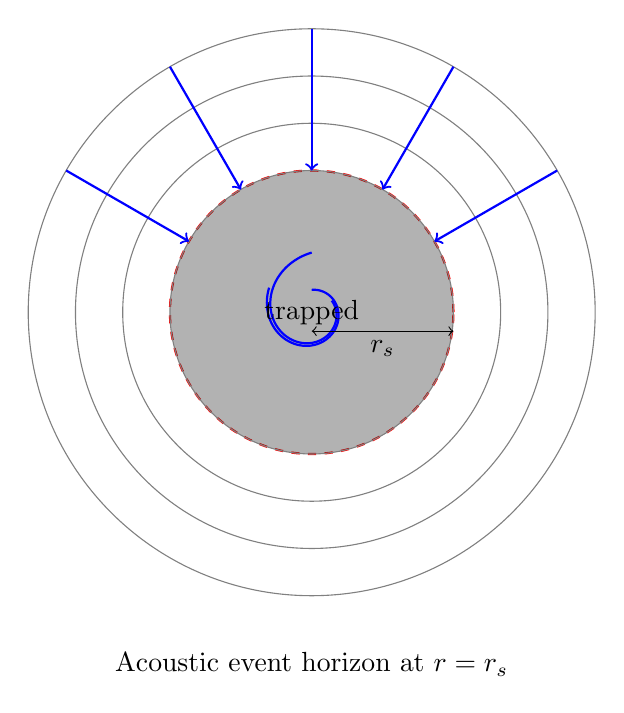
\begin{tikzpicture}[scale=1.2]
  % Horizon
  \draw[thick, dashed, red] (0,0) circle (1.5cm);
  \fill[black, opacity=0.3] (0,0) circle (1.5cm);

  % Radial grid
  \foreach \r in {1.5, 2.0, 2.5, 3.0}
    \draw[thin, gray] (0,0) circle (\r cm);

  % Incoming sound rays
  \foreach \angle in {30, 60, 90, 120, 150}
  {
    \draw[->, thick, blue] ({3*cos(\angle)}, {3*sin(\angle)})
      -- ({1.5*cos(\angle)}, {1.5*sin(\angle)});
  }

  % Spiraling trapped rays
  \draw[thick, blue, domain=150:450, samples=100]
    plot ({1.3*cos(\x)/(1+0.01*\x)}, {1.3*sin(\x)/(1+0.01*\x)});
  \draw[thick, blue, domain=90:390, samples=100]
    plot ({1.2*cos(\x)/(1+0.01*\x)}, {1.2*sin(\x)/(1+0.01*\x)});

  % Labels
  \node at (0,0) {trapped};
  \node[below] at (0,-3.5) {Acoustic event horizon at $r = r_s$};
  \draw[<->] (0,-0.2) -- (1.5,-0.2) node[midway, below] {$r_s$};
\end{tikzpicture}
\end{center}

The surface gravity at the horizon is $\kappa_H = c_0/(2r_s)$, giving Hawking
temperature:

\margindim{For $c_0 = 340$ m/s (air) and $r_s = 1$ cm, the Hawking temperature
is $T_H \sim 10^{-8}$ K---undetectable. In BEC systems with $c_s \sim 1$ mm/s
and $r_s \sim 10\,\mu$m, $T_H \sim 1$ nK, within experimental reach.}

\begin{equation}
T_H = \frac{\hbar \kappa_H}{2\pi k_B} = \frac{\hbar c_0}{4\pi k_B r_s}
\end{equation}

%------------------------------------------------------------------------------
% Section 4: Fractal Antennas and Self-Similarity
%------------------------------------------------------------------------------

\section{Fractal Antennas and Multiband Response}

Fractal geometries---self-similar structures that repeat patterns across
scales---provide a natural framework for designing antennas that operate
efficiently at multiple frequencies. The key insight is that a fractal
structure contains features at many length scales, each resonating at a
different frequency.

\marginhistory{Fractal antennas were pioneered by Nathan Cohen in the 1980s,
initially for the Manta dual-band array. The Sierpinski gasket antenna
emerged in the mid-1990s, demonstrating multiband behavior with a single
compact element.}

\subsection{The Sierpinski Gasket Antenna}

The Sierpinski triangle is constructed by iterative subdivision: start with
an equilateral triangle, remove the central inverted triangle, then repeat
the process on each of the three remaining triangles. After $n$ iterations,
the structure contains $3^n$ triangular elements.

An antenna built from a Sierpinski gasket with side length $a$ exhibits
resonances at wavelengths:

\begin{equation}
\lambda_n = \frac{2a}{n} \cdot \log_3(2)^n
\end{equation}

approximately, for $n = 1, 2, 3, \ldots$. The $\log_3(2) \approx 0.63$ scaling
reflects the fractal dimension $D = \log_3(2) \approx 1.585$.

\marginmath{The Hausdorff dimension of the Sierpinski gasket is
$D = \log(N)/\log(s)$ where $N=3$ is the number of self-similar pieces and
$s=2$ is the scaling factor. Thus $D = \log(3)/\log(2) \approx 1.585$, between
a line ($D=1$) and a filled triangle ($D=2$).}

\begin{center}
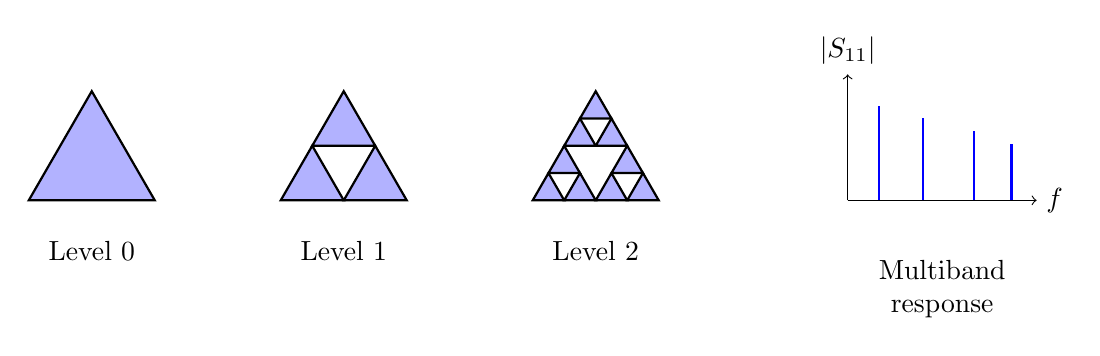
\begin{tikzpicture}[scale=0.8]
  % Level 0: Full triangle
  \begin{scope}[shift={(-6,0)}]
    \draw[thick, fill=blue!30] (0,0) -- (2,0) -- (1,1.732) -- cycle;
    \node[below] at (1,-0.5) {Level 0};
  \end{scope}

  % Level 1: Remove center
  \begin{scope}[shift={(-2,0)}]
    \draw[thick, fill=blue!30] (0,0) -- (1,0) -- (0.5,0.866) -- cycle;
    \draw[thick, fill=blue!30] (1,0) -- (2,0) -- (1.5,0.866) -- cycle;
    \draw[thick, fill=blue!30] (0.5,0.866) -- (1.5,0.866) -- (1,1.732) -- cycle;
    \node[below] at (1,-0.5) {Level 1};
  \end{scope}

  % Level 2: Further subdivision
  \begin{scope}[shift={(2,0)}]
    % Bottom left
    \draw[thick, fill=blue!30] (0,0) -- (0.5,0) -- (0.25,0.433) -- cycle;
    \draw[thick, fill=blue!30] (0.5,0) -- (1,0) -- (0.75,0.433) -- cycle;
    \draw[thick, fill=blue!30] (0.25,0.433) -- (0.75,0.433) -- (0.5,0.866) -- cycle;
    % Bottom right
    \draw[thick, fill=blue!30] (1,0) -- (1.5,0) -- (1.25,0.433) -- cycle;
    \draw[thick, fill=blue!30] (1.5,0) -- (2,0) -- (1.75,0.433) -- cycle;
    \draw[thick, fill=blue!30] (1.25,0.433) -- (1.75,0.433) -- (1.5,0.866) -- cycle;
    % Top
    \draw[thick, fill=blue!30] (0.5,0.866) -- (1,0.866) -- (0.75,1.299) -- cycle;
    \draw[thick, fill=blue!30] (1,0.866) -- (1.5,0.866) -- (1.25,1.299) -- cycle;
    \draw[thick, fill=blue!30] (0.75,1.299) -- (1.25,1.299) -- (1,1.732) -- cycle;
    \node[below] at (1,-0.5) {Level 2};
  \end{scope}

  % Frequency response
  \begin{scope}[shift={(7,0)}]
    \draw[->] (0,0) -- (3,0) node[right] {$f$};
    \draw[->] (0,0) -- (0,2) node[above] {$|S_{11}|$};

    % Resonance peaks
    \draw[thick, blue] (0.5,0) -- (0.5,1.5);
    \draw[thick, blue] (1.2,0) -- (1.2,1.3);
    \draw[thick, blue] (2.0,0) -- (2.0,1.1);
    \draw[thick, blue] (2.6,0) -- (2.6,0.9);

    \node[below, text width=2.5cm, align=center] at (1.5,-0.8) {Multiband response};
  \end{scope}
\end{tikzpicture}
\end{center}

\subsection{Optimization and Performance}

For a Sierpinski gasket with base side $a = 10$ cm, the first three resonances
occur at approximately:

\marginex{A practical implementation uses a printed circuit board with copper
traces forming the fractal pattern. Feeding the antenna from one vertex,
resonances appear at 900 MHz (GSM), 1.8 GHz (PCS), and 2.4 GHz (WiFi) for
$a \approx 8$ cm.}

\begin{align}
f_1 &\approx \frac{c}{2a} = 1.5\,\text{GHz} \\
f_2 &\approx \frac{c}{2a} \cdot 2^{1.585} \approx 4.5\,\text{GHz} \\
f_3 &\approx \frac{c}{2a} \cdot 3^{1.585} \approx 10.8\,\text{GHz}
\end{align}

The radiation efficiency at each band depends on the ohmic losses and the
effective aperture. For a well-designed fractal antenna, the gain ranges from
2--5 dBi across all bands, with input impedance matching achieved through
fractal self-similarity.

The volume occupied by the antenna scales as $V \sim a^D$ where $D$ is the
fractal dimension. This enables compact designs: a fractal antenna with
$D = 1.585$ occupies only $a^{1.585}$ volume compared to $a^3$ for a Euclidean
structure, a reduction factor of $a^{1.415}$ for large $a$.

\margincomp{Genetic algorithms and particle swarm optimization can evolve
fractal geometries beyond standard forms like Sierpinski or Koch curves,
discovering application-specific designs with superior bandwidth and gain
characteristics.}

%------------------------------------------------------------------------------
% Conclusion
%------------------------------------------------------------------------------

\section{Conclusion}

Metamaterial engineering realizes the fundamental principle that material
structure and spacetime geometry are two sides of the same coin. By sculpting
permittivity, permeability, density, and elasticity as functions of position
and frequency, we create effective metrics that guide wave propagation along
prescribed paths.

\marginxref{The techniques developed here connect directly to the geometric
frameworks of Papers 1--3. The effective metrics are fiber bundles over
configuration space, with gauge fields encoding the material response. Fractal
antennas probe the self-similar structures explored in Paper 3.}

Transformation optics enables cloaking devices, perfect lenses, and field
concentrators. Acoustic metamaterials simulate black hole physics in the
laboratory, probing quantum effects at horizons. Fractal geometries compress
multiband functionality into compact structures, exploiting self-similarity
across scales.

These are not mere analogies. The mathematics is identical: Maxwell's equations
in a metamaterial and Einstein's equations in curved spacetime share the same
geometric foundation. The metamaterial designer is, quite literally, an
architect of spacetime---at least from the perspective of the waves propagating
through their creation.

The next chapter turns to speculative frontiers: warp drives, wormholes, and
Planck-scale engineering, asking what technologies might emerge if the principles
developed throughout this series can be pushed to their ultimate limits.

%==============================================================================
% END OF CHAPTER 3
%==============================================================================
